%%%%%%%%%%%%%%%%%%%%%%%%%%%%%%%%%%%%%%%%%%%%%%%%%%%%%%%%%%%%%%%%%%%%%%%%%%%%%%%%%%%%%%%%%%%%%
%%									Chapitre 2												%
%%%%%%%%%%%%%%%%%%%%%%%%%%%%%%%%%%%%%%%%%%%%%%%%%%%%%%%%%%%%%%%%%%%%%%%%%%%%%%%%%%%%%%%%%%%%%

\chapter{Imagerie morphologique de la circulation intracr\^anienne}
\label{chap:imageriemorpho}	
\minitoc


%%%%%%%%%%%%%%%%%%%%%%%%%%%%%%%%%%%%%%%%%%%%%%%%%%%%%%%%%%%%%%%%%%%%%%%%%%%%%%%%%%%%%%%%%%%%%



% Début du chapitre

Dans ce chapitre nous allons décrire comment l’imagerie IRM permet de reconstruire, pour un sujet ou un patient, une partie de l’anatomie du système circulant intracrânien. Dans un premier temps nous ferons une revue anatomique détaillée. En effet il est nécessaire, pour motiver toute simplification ultérieure, de s’appuyer sur la description la plus complète possible des données anatomiques. Dans une deuxième partie nous nous intéresserons aux outils d’imagerie IRM disponibles. Notre objectif sera, en référence à la description anatomique complète, de mettre en évidence le degré de précision actuel auquel peut descendre l’imagerie en termes de données de morphologie quantitative, de façon à adapter à ces données notre modèle biophysique.

%%%
\begin{figure}[!t]
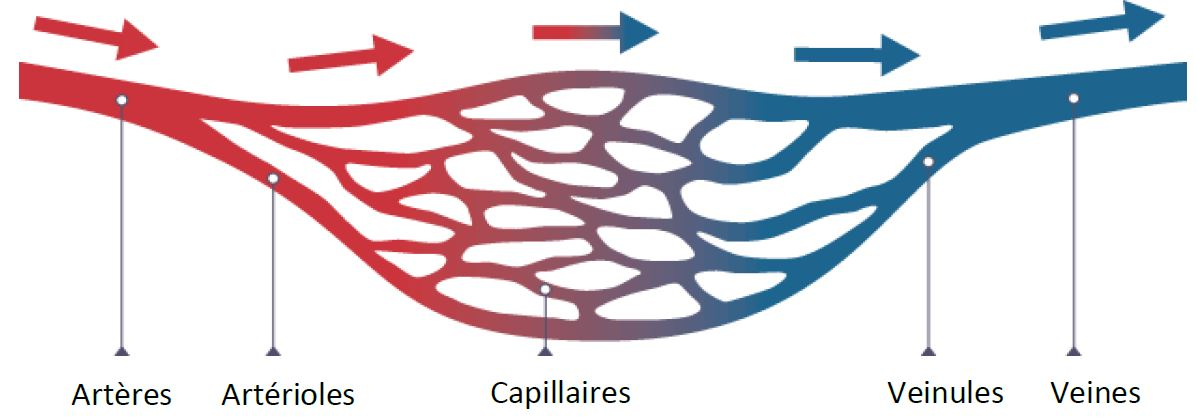
\includegraphics[width=\linewidth]{1_1_schema_arteres_cap_veines}
\caption{Schéma de l'organisation structurale d'une branche du système sanguin.}
\label{fig:1_1_schema_arteres_cap_veines}	
\end{figure}
%%%
\section{Anatomie}
Les vaisseaux sanguins ont plusieurs fonctions. Ils permettent d’apporter les nutriments et l’oxygène nécessaire au bon fonctionnement des organes, tout en étant les porteurs des messagers hormonaux à grande distance dans l’organisme. La même structure simple de circulation sanguine se reproduit dans tous les tissus (Figure~\ref{fig:1_1_schema_arteres_cap_veines}). Les artères amènent le sang oxygéné vers les muscles (dans notre cas le cerveau), ces artères se divisent en artérioles de calibres moins importants et capables d’assurer le contrôle du débit, pour enfin arriver aux capillaires, lieu d’échange moléculaire avec le tissu environnant. Le sang désoxygéné est ensuite évacué vers les veinules puis veines.
Au niveau cérébral, nous retrouvons cette structure artères, capillaires, veines. Notons que les systèmes artériels et veineux ne sont pas symétriques.

\subsection{Artères et artérioles}
\label{sec:anat_art}
\subsubsection{Architecture}
Le cerveau est extrêmement dépendant de la circulation cérébrale du fait de son métabolisme élevé que manifeste sa sensibilité à l’ischémie (apport insuffisant de sang). La régularité de l’apport en sang dans le cerveau est assurée par plusieurs mécanismes. Structuralement, la présence de {\em vaisseaux collatéraux} fournit des voies d’accès parallèles au tissu cérébral. Dynamiquement, un système précis d’{\em autorégulation}  impliquant des phénomènes de {\em vasodilatation} et {\em vasoconstriction} régule en permanence le débit.

On distingue morphologiquement et physiologiquement les circulations {\em antérieures} et {\em postérieures}. 

Du côté de la circulation antérieure, le sang est délivré au cerveau par l’intermédiaire des deux {\em carotides internes} (Figure~\ref{fig:1_2_poly_willis}). Chaque carotide interne bifurque pour former une {\em artère cérébrale moyenne} (ACM) et une {\em artère cérébrale antérieure} (ACA), allant perfuser respectivement les régions {\em temporales} et {\em pariétales} d’une part et les régions {\em frontales} de l’autre. 

L’{\em artère cérébrale antérieure} se dirige en avant et en dedans, passe au-dessus du nerf optique et se rapproche de celle du côté opposé pour lui devenir parallèle et pénétrer dans la scissure qui sépare les deux hémisphères cérébraux. Elle contourne l'extrémité antérieure du corps calleux pour se diriger d'abord en haut, puis en haut et en arrière, et enfin en arrière et en bas, en suivant toute la surface supérieure du corps calleux. Elle se termine par trois branches : antérieure, moyenne et postérieure qui vont vasculariser la face interne des lobes frontaux et pariétaux, débordant sur la face externe, ainsi que le bord supérieur et l'extrémité antérieure de la face externe des hémisphères cérébraux.

L'{\em artère cérébrale moyenne} irrigue en superficie la majeure partie de la surface latérale de l'hémisphère, en dehors de l'extrémité supérieure des lobes frontaux et pariétaux et de la partie inférieure du lobe temporal ; en profondeur, les ganglions de la base et la capsule interne.

Du côté de la {\em circulation postérieure}, l’entrée se fait par les deux {\em artères vertébrales} (VA). Elles se rejoignent pour former l’{\em artère basilaire}, qui se divise à son tour pour donner les {\em artères cérébrales postérieures gauches} et {\em droites} (ACP). Les branches {\em perforantes} de l'artère cérébrale postérieure sont à destination du thalamus et de la paroi du troisième ventricule. Les branches {\em choroïdiennes} irriguent le troisième ventricule, les plexus choroïdes, le pédoncule cérébral, le fornix, le thalamus et le noyau caudé. Les branches {\em corticales} vascularisent les lobes temporaux et occipitaux.

Les circulations postérieures et antérieures sont interconnectées par les {\em artères communicantes antérieures} et {\em postérieures} (ACoA et PCoA). Il en résulte une structure en forme d’anneau, appelée le {\em polygone ou cercle de Willis} (CoW, voir figure ~\ref{fig:1_2_poly_willis}).
%%%
\begin{figure}[!t]
\centering
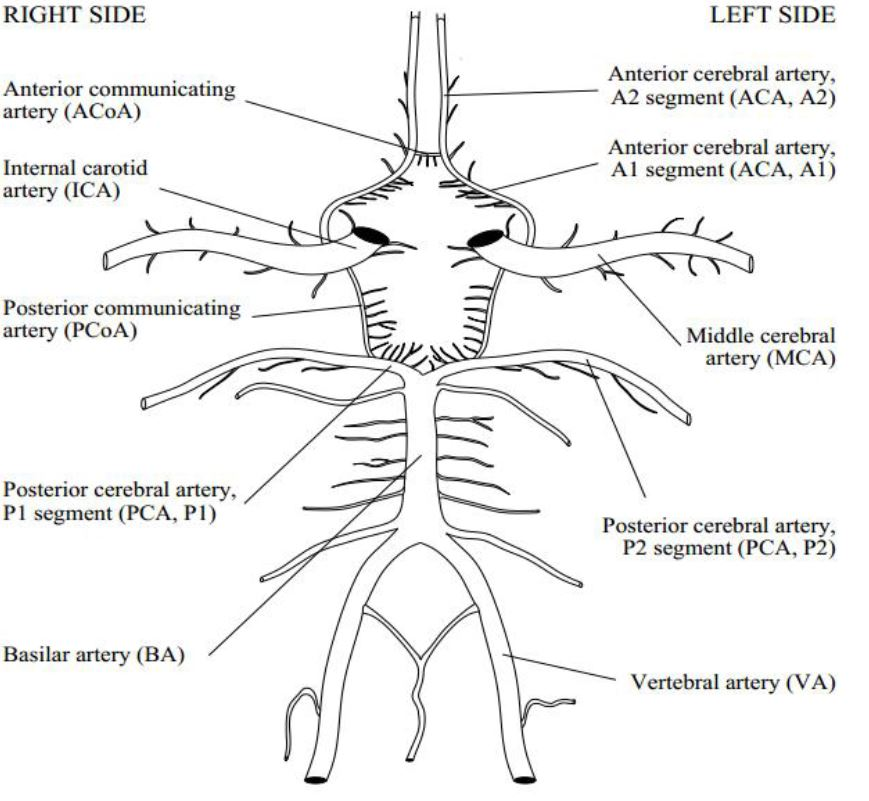
\includegraphics[width=12cm]{1_2_poly_willis}
\caption{Représentation schématique du polygone de Willis. }
\label{fig:1_2_poly_willis}	
\end{figure}
%%%
Cette structure est la voie collatérale principale de la circulation cérébrale, elle fournit un apport parallèle de sang aux artères efférentes en cas de vaisseaux manquants ou bouchés (\cite{Alastruey2007}). Le cerveau représente 2\% du poids total du corps humain, pourtant, il représente 20\% de la consommation totale en oxygène et 25\% de la consommation en glucose. Il est ainsi crucial de maintenir un apport constant et coordonné à l’activité neuronale. Le système artériel est principalement conducteur, c’est-à-dire qu’il amène le sang vers le cerveau. La présence du polygone de Willis permet de protéger en partie ce dernier. Les artères communicantes permettent d'alimenter des artères cérébrales par une source qui n'est pas l'artère habituelle. Ainsi, on peut vivre avec une carotide bouchée, car le sang passe tout de même dans les artères cérébrales qu'elle est censée desservir, en passant par le tronc basilaire ou l'artère communicante antérieure. Certaines occlusions ne peuvent cependant pas être compensées. Une anomalie du cercle de Willis n'est pas un danger en soi, mais rend un éventuel accident vasculaire plus dangereux.

Il existe une grande variabilité anatomique du polygone de Willis (figure ~\ref{fig:1_3_willis_variations}). 
%%%
\begin{figure}[!t]
\centering
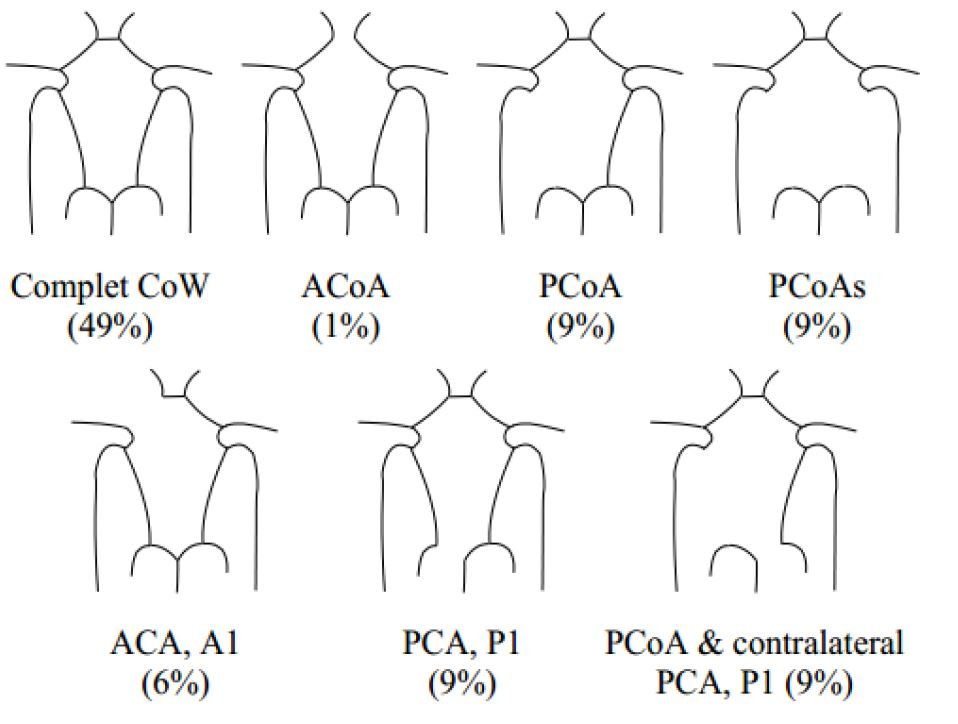
\includegraphics[width=12cm]{1_3_willis_variations}
\caption{Représentation schématique des variations individuelles décrites pour la structure du polygone de Willis (\cite{LippertPabst1985}). }
\label{fig:1_3_willis_variations}	
\end{figure}
%%%
Sur la base de plus de 50 études anatomiques et radiologiques, Lippert et Pabst (\cite{LippertPabst1985}) ont montré que près de 50 \% de la population dispose d’un polygone de Willis avec au moins une artère absente, très petite ou incomplètement développée (hypoplasique) (Figure~\ref{fig:1_3_willis_variations}). Ces variations anatomiques réduisent la disponibilité des artères collatérales et augmentent le risque d’accident vasculaire cérébral (AVC) et d’accident ischémique transitoire (AIT) chez les patients (\cite{Henderson2000}).

D’autres systèmes d’anastomoses sont présents au niveau du cerveau comme entre les artères cérébrales à la surface du cortex mais sont considérées comme peu efficaces.

\subsubsection{Microstructure}

Les artères et artérioles sont constituées de trois couches appelées {\em adventice},  {\em média} et  {\em intima}. Leur importance varie en fonction du type de vaisseau.

L’ {\em adventice} est composée de tissu de connexion lâche dans lequel se terminent des fibres nerveuses amyéliniques. Une lame élastique externe peut être mise en évidence entre l’adventice et la média des artères cérébrales et des artères pie-mériennes.

La  {\em média} est constituée de  {\em cellules musculaires lisses} (SMC) responsables de la vasomotricité. Elles sont présentes dans les artères cérébrales, les artères pie-mériennes et les artérioles. Leur nombre diminue lorsque le diamètre des vaisseaux décroit.

L’ {\em intima} enfin est formée d’une monocouche de cellules endothéliales qui sont jointives par l’intermédiaire de  {\em jonctions serrées}. Ces jonctions séparent le cerveau du sang par une barrière dite  {\em barrière hémato-encéphalique} (Blood Brain Barrier, BBB). La BBB a une perméabilité sélective pour les molécules lipophiles à faible poids moléculaire et pour celles qui possèdent un transporteur spécifique. Toutefois, les capillaires de certaines régions situées près des ventricules, de l'éminence médiane, de la glande pinéale et de la neurohypophyse entre autres sont fenestrés . Les substances sanguines peuvent alors atteindre le liquide extracellulaire et les neurones, flux dont la modélisation devra tenir compte. En sens inverse, les neurohormones peuvent être déversées dans la circulation qui les transportera vers leurs cibles.

Les artères se caractérisent par une média épaisse. Les artérioles, elles, représentent le site primaire de la résistance vasculaire, ce sont des vaisseaux de faible diamètres (<0.5 mm) disposant d’une paroi épaisse. L’intima est réduite à l’endothélium reposant sur la membrane basale. La média est très musculaire et innervée par le système nerveux sympathique. L’adventice lui, se fond dans le tissu conjonctif environnant. Leur diamètre peut être modifié en fonction de plusieurs facteurs (molécules circulantes, pH, contraintes mécaniques etc.). Les artérioles jouent ainsi un rôle important dans le contrôle du débit sanguin.

%%%
%%%
\subsubsection{Données quantitatives}
Les données quantitatives relatives à la {\em longueur} et au {\em diamètre} sont sujettes à de fortes variabilités individuelles, comme on l'a vu précédemment pour la structure du polygone de Willis. Dans notre travail, nous nous fixerons comme objectif de les reconstruire pour chaque sujet. Cependant, à titre de référence, le projet {\em BraVa}, pour {\em The Brain Vasculature}, fournit une base de données relatives à l'architecture artérielle dans le cerveau (\cite{Wright2013}). Pour construire cette base, 61 patients (âge 31.16 $\pm$10.03) ont subit une imagerie IRM par temps de vol (résolution 0.6 x 0.6 x 0.6mm$^3$) . Pour chaque sujet, une identification manuelle des artères a été réalisée via ImageJ et le plugin Neuron\_Morpho (\cite{neuronmorpho}). Ainsi une identification fine du nombre de segments et de leurs caractéristiques (longueur, tortuosité etc.) est disponible et mis à disposition en ligne. Cette base nous renseigne entre autre sur le nombre de branches du système artériel et les longueurs moyennes. Ainsi le système artériel tel qu'identifié par BraVa consiste en moyenne chez les sujets en 208.56 branches pour des longueurs allant de 27 à 43 mm avec une valeur moyenne à 34.18 mm.

Le tableau~\ref{tab:databrava} récapitule les données issues de ce travail de morphologie quantitative pertinentes pour nous. Les longueurs des {\em artères cérébrales antérieures}, {\em artères cérébrales moyennes} et {\em artères cérébrales postérieures} sont disponibles (branches {\em droites} et {\em gauches}) pour chacun des 61 sujets. L'ampleur de la variabilité individuelle en termes de longueurs de ces artères renforce clairement la volonté de construire une modélisation sujet-spécifique. Ces données permettent tout de même de disposer d'{\em ordres de grandeur} permettant de vérifier la pertinence de nos segmentations. Nous observons ainsi après comparaison avec une segmentation manuelle réalisée sur nos données de couverture anatomique similaire à BraVa, des résultats concordants.

%%%
\begin{table}
\caption{Longueur des {\em artères cérébrales antérieures}, {\em artères cérébrales moyennes} et {\em artères cérébrales postérieures} telles que mesurées dans le projet BraVa pour 61 sujets (données extraites de la base BraVa en ligne \textcolor{red}{\tt cng.gmu.edu/brava/}). Des mesures extraites d'une segmentation manuelle (voir~\ref{sec:segmentation} et figure~\ref{fig:2_comparaisons_segmentations}) sur un TOF de couverture anatomique similaire à BraVa sont données à titre de comparaison.}
\label{tab:databrava}
\begin{tabularx}{\linewidth}{|X| X X X X X|}
\hline
\centering
      & Longueur mesurée (mm) &  Longueur Moyenne BraVa (mm) &  Déviation Standard (mm) & Minimum (mm) & Maximum  (mm)\\
 \hline
   {\small Artère Cérébrale Antérieure gauche} & 525 &  {\bf 865.02}	&194.74	&318.14	&1295.80 \\
\hline
    {\small Artère Cérébrale Antérieure droite} & 525 & {\bf  889.70}	& 205.38	&233.96	&1344.20 \\
\hline
    {\small Artère Cérébrale Postérieure gauche} & 309 &  {\bf 492.96}	&118.13	&227.87	&747.71 \\
\hline
   {\small Artère Cérébrale Postérieure droite } & 344 & {\bf 508.69}	&128.30	&245.07	&770.19\\
\hline
   {\small Artère Cérébrale Moyenne gauche} &   1862	&{\bf  1899.90}	&294.24	&1271.74	&2635.63 \\
\hline
   {\small Artère Cérébrale Moyenne  droite} &  1662 &{\bf 1856.52}	&296.41	&966.78	&2507.67 \\
   
\hline

\end{tabularx}
\end{table}




Les artérioles, quand à elles, ne pourront en général pas être reconstruites à l'aide des techniques d'imagerie disponibles. Il nous faudra donc considérer des longueurs et des diamètres moyens issus de la littérature ou estimés. On considère en général que les artérioles ont des diamètres internes de 30 $\mu$m ou moins (\cite{Martini2009}).

\subsection{Microcirculation}
\label{sect:microcirculation}
En raison du caractère invasif des techniques requises pour son étude, les caractérisations de la microanatomie chez l’homme sont rares (\cite{Brett2002}) et il n’existe dans la littérature que peu de données quantitatives sur la microvascularisation cérébrale. Néanmoins une étude récente au moins a permis une caractérisation morphologique de cette microcirculation (\cite{Lauwers2008}). Il a ainsi été observé une taille moyenne des capillaires de 6.47 $\mu$m de diamètre pour une longueur de 52.95 $\mu$m et ce avec une remarquable constance. On considère de manière générale que les capillaires sont des vaisseaux de diamètre inférieur à 10 $\mu$m. L’organisation topologique des capillaires ne fait pas l’objet d’un consensus clair notamment entre organisation en {\em réseau}, et organisation en {\em arbre}. Il semble néanmoins admis que les capillaires s’organisent préférentiellement en réseau de façon à ce que tout soit connecté, c’est-à-dire que l’ensemble du réseau puisse être complètement perfusé quelle que soit l’entrée. Quelques structures en arbre avec une entrée de subdivisant en plusieurs vaisseaux ont malgré tout été observées.

Les capillaires représentent des réseaux denses avec une densité de longueur moyenne de 500 mm/mm$^3$ de parenchyme. Des variations de cette valeur sont observées entre la surface du cerveau (613 mm/mm$^3$) et le bas de la scissure (411 mm/mm$^3$)  (\cite{Lauwers2008}). Cela est lié à l’orientation opposée des plis dans ces territoires : la contraction au sommet du gyrus induit géométriquement une augmentation de la densité. La surface d’échange chez l’homme (mesuré par la surface vasculaire par mm$^3$) semble être plus importante que chez le primate (11.74 mm$^2$/mm$^3$ versus 4.5 mm$^2$/mm$^3$) (\cite{Lauwers2008},~\cite{Risser2007}). Enfin, le volume vasculaire par mm$^3$, qui permet d’estimer le volume sanguin cortical, est de l’ordre de 2.4\% à 3\% selon le territoire.

Ces données fournissent une description géométrique quantitative cohérente de la structure des capillaires. Pour chaque mm$^3$, on a 500 mm de capillaires, ce qui pour un diamètre typique inférieur a 10 $\mu$m, donne bien un volume inférieur à 5\% et une surface de 10 mm$^2$ d'échange. Structuralement, si on suppose une organisation réticulée, cubique pour simplifier les calculs, on aboutit à un réseau de 20 unités de coté, soit du point de vue hydrodynamique 400 tubes de 10 $\mu$m de diamètre en parallèle. Ces chiffres sont évidemment en l'état de l'imageire  microstructurale très aproximatifs. 

Du point de vue microstructural, les capillaires ne présentent pas de tissu conjonctif périvasculaire, remplacé par les prolongements astrocytaires. On peut noter la présence de jonctions serrées réunissant les cellules endothéliales, et d’un équipement enzymatique riche et parfois spécifique. Les capillaires permettent de fournir les nutriments et le dioxygène aux tissus. Ils jouent un rôle important dans le contrôle du passage des molécules : les macromolécules ne franchissent pas la barrière hématotissulaire tandis que pour les petites molécules la perméabilité est identique à celle de la membrane cellulaire. Ils permettent le passage libre des molécules lipophiles mais requierent l’utilisation de transporteurs membranaires, parfois spécifiques, pour les molécules hydrophiles. Enfin ils assurent le contrôle du passage des cellules, en le réduisant au renouvellement lent mais constant des cellules microgliales par des précurseurs dérivant de la moelle osseuse.

\subsection{Veines}
L'union de plusieurs capillaires donne des {\em veinules} qui elles-mêmes se déversent dans des {\em veines} de diamètre croissant. Habituellement on classe les veines en fonction de leur taille. Dans l'espèce humaine, les petites veines ont un diamètre compris entre 50 $\mu$m et 1 mm; les veines moyennes ont un diamètre compris entre 1 mm et 10 mm et les larges veines ont plus d'un centimètre de diamètre. Les veinules ont le même aspect que les capillaires, mais leur diamètre est supérieur (inférieur à 50$\mu$m - \cite{Martini2009}).

Comme les capillaires, les veinules interviennent dans les échanges métaboliques. Leur principale caractéristique est leur sensibilité aux agents inflammatoires qui augmentent leur perméabilité, ce qui permet la diffusion du plasma et le passage de protéines de haut poids moléculaire. Ces agents favorisent aussi l'adhérence des leucocytes aux parois vasculaires et leur diapédèse (intercalation entre les cellules endothéliales), en ralentissant le flux sanguin. Les veines enfin disposent d’une structure similaire aux artères mais avec une lumière plus grande, une paroi plus fine avec peu d’éléments musculaires et élastiques dans la média.

Le système veineux cérébral est un système interconnecté et communiquant librement, composé des {\em sinus veineux} et des {\em veines cérébrales} (\cite{Schaller2004}). Les veinules du réseau post-capillaire se regroupent en veines cheminant dans la substance blanche (veines médullaire) qui vont converger vers la surface de l'encéphale pour donner naissance à deux systèmes de veines regroupées, appelés {\em système superficiel} et {\em système profond}. Compte tenu de leur importance dans la modélisation des flux intracr\^aniens, on va en faire une description détaillée issue de~\cite{radioanatDrainage}.

Le système superficiel (cortical) draine le sang du cortex et de la matière blanche sous corticale (\cite{Aydin1997}). Les veines dites superficielles ou corticales cheminent à la surface de l’encéphale et vont gagner (directement ou indirectement) par l’intermédiaire de veines collectrices plus volumineuses, un sinus veineux. Ainsi les veines corticales proches de la convexité haute se jettent directement dans le {\em sinus sagittal supérieur}, les veines des faces inférieures et latérales de l’encéphale forment des collecteurs plus volumineux (veines {\em sylviennes} en avant et latéralement, veines {\em basales} en dedans et en arrière) rejoignant soit le système profond (veines basales), soit directement un sinus.

%%%
\begin{figure}[!t]
\centering
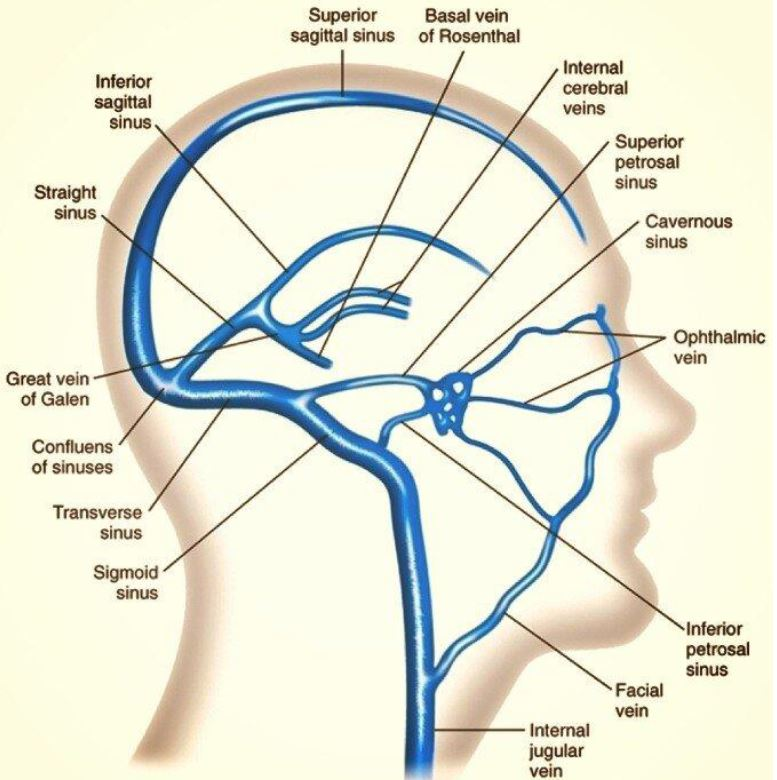
\includegraphics[width=12cm]{1_4_syst_veineux}
\caption{Structure des sinus veineux, {\em Elsevier Inc.} }
\label{fig:1_4_syst_veineux}	
\end{figure}
%%%
Le système profond ({\em médullaire} et {\em sous épendymaire}) draine les structures profondes et médianes du cerveau (commissures interhémisphériques, noyaux gris, système ventriculaire). Il est essentiellement constitué par les deux veines cérébrales internes cheminant d’avant en arrière sur la toile choroïdienne du 3ème ventricule et le bord inférieur du splenium du corps calleux. Chacune des veines cérébrales internes s’unit en arrière à son homologue controlatérale pour donner au point le plus déclive du splenium du corps calleux la {\em grande veine de Galien}.

On observe différents sinus veineux (Figure~\ref{fig:1_4_syst_veineux}). Tout d’abord le {\em sinus sagittal supérieur} (SSS) contenu dans un dédoublement de l’insertion supérieure de la faux du cerveau en position médiane, reçoit les veines corticales des régions fronto-pariéto-occipitales supéro-externe et interne du cerveau. Il se termine dans la région occipitale médiane au niveau d’une structure particulière appelée {\em torcular} ou {\em pressoir d’Hérophile} en deux sinus latéraux. Les sinus latéraux vont cheminer dans l’insertion de la grande circonférence de la tente du cervelet au niveau de la voûte occipitale. Chaque sinus latéral rejoint la région temporo-occipito-pétreuse latérale, puis par un trajet descendant sigmoïde dans le dièdre squamo-pétreux, va gagner la partie veineuse du foramen jugulaire et donner naissance à l’origine du golfe de la veine jugulaire interne.

Le {\em sinus sagittal inférieur}, d’importance moindre, chemine dans un dédoublement de la partie inférieure libre de la faux du cerveau, d’avant en arrière pour gagner le sinus droit. Ce dernier est contenu dans l’insertion de la faux du cerveau sur la tente du cervelet en position médiane. Il se jette, après avoir reçu la veine de Galien, dans le pressoir d’Hérophile, zone de confluence entre sinus sagittal supérieur, sinus droit et origine des deux sinus latéraux.

Enfin, les {\em sinus veineux de la base du crâne} cheminent dans un dédoublement de la partie inférieur libre de la faux du cerveau, d’avant en arrière, pour gagner différents sinus (Figure~\ref{fig:1_5_sinus_veineux}). 
%%%
\begin{figure}[!t]
\centering
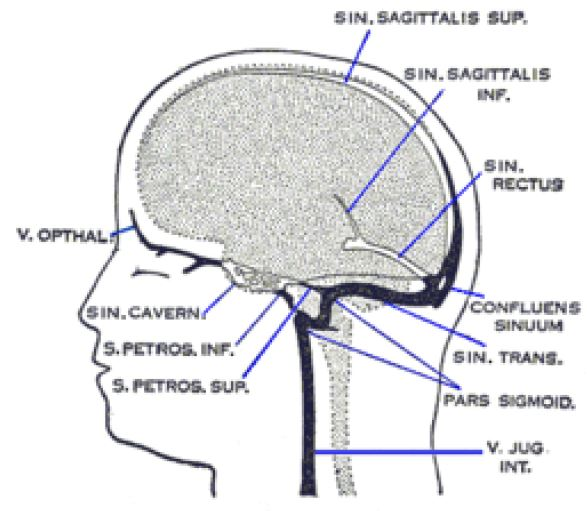
\includegraphics[width=10cm]{1_5_sinus_veineux}
\caption{Illustration des sinus de la base du cr\^ane, {\em Anatomie de Gray (1858)}. }
\label{fig:1_5_sinus_veineux}	
\end{figure}
%%%
Le {\em sinus caverneux}, situé de part et d’autre de la loge hypophysaire contre la face latérale du corps du sphénoïde, dans lequel chemine l’artère carotide interne. Le {\em sinus sphéno-pariétal de Breschet}, qui draine les veines méningées moyennes et parfois la veine sylvienne. En arrière le sinus caverneux se draine dans le {\em sinus pétreux inférieur}, cheminant dans la suture sphéno-pétreuse en haut, pétro-occipitale en bas, et rejoignant à la face inférieure de la base du crâne le golfe de la jugulaire. En arrière et latéralement, le {\em sinus pétreux supérieur}, contenu dans l’insertion pétreuse de la grande circonférence de la tente du cervelet, au niveau du bord supérieur du rocher, se termine au niveau du tiers externe de celui-ci en s’abouchant dans le sinus latéral.

Contrairement aux artères où l’on observe peu de suppléance vasculaire (hors polygone de Willis), le système veineux s’anastomose beaucoup. Les sinus pétreux anastomosent la circulation veineuse antérieure et postérieure. Le sinus sagittal supérieur et la veine cérébrale moyenne s’anastomosent par la {\em grande veine anastomotique de Trolard}. La veine cérébrale moyenne avec le sinus transverse par la {\em veine anastomotique de Labbé}. Des anastomoses existent aussi entre les sinus caverneux par les sinus inter caverneux antérieur et postérieur.

Du point de vue de la modélisation, les compartiments veineux seront, comme les compartiments artériels, reconstruits sur la base d'une analyse morphologique sujet-spécifique. Dans ce cas, aucun travail de morphologie quantitative comparable au projet BraVa ne pourra nous fournir de référence. Comme les artérioles, les veinules ne pourront pas être segmentées, et des hypothèses issues de la littérature devront être proposées pour leur longueur et leur densité caractéristique.  
\subsection{Liquide cérébro-spinal}
Le liquide cérébro-spinal est un liquide biologique transparent dans lequel baigne le cerveau. Il est contenu dans les méninges entre la pie-mère qui recouvre le système nerveux central et l’arachnoïde qui tapisse le versant interne de la dure-mère, c’est-à-dire dans l’espace sous-arachnoïdien.

Le cerveau comprend des cavités remplies de liquide céphalorachidien. Ce réseau de canaux situé à l’intérieur du cerveau forme le système ventriculaire (Figure~\ref{fig:1_6_systeme_ventriculaire}).
%%%
\begin{figure}[!t]
\centering
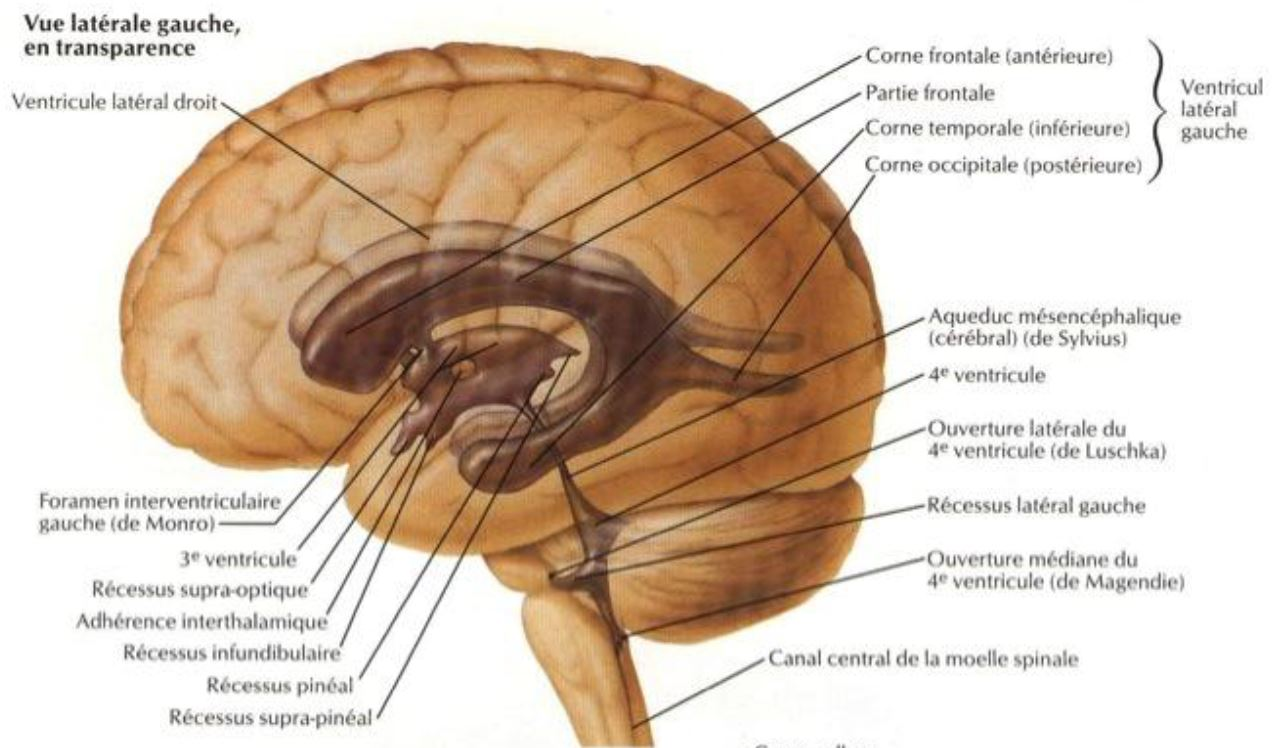
\includegraphics[width=15cm]{1_6_systeme_ventriculaire}
\caption{Système ventriculaire du cerveau,  {\em neurochirurgie-cedres.com}. }
\label{fig:1_6_systeme_ventriculaire}	
\end{figure}
%%%
Il y a en tout quatre ventricules.

Le deux premiers ventricules cérébraux, sont habituellement appelés {\em ventricules latéraux}. Ils sont situés en profondeur dans chacun des deux hémisphères cérébraux. Ils présentent une forme de fer à cheval, orientée d'arrière en avant. Chaque ventricule possède une {\em corne frontale} (en avant) située dans le lobe frontal de l'hémisphère cérébral correspondant, une branche inférieure ({\em corne temporale}, sur les côtés du cerveau), une partie postérieure appelée {\em carrefour} qui rassemble les branches inférieures et supérieures, et enfin une petite zone supplémentaire, appelée {\em corne occipitale}, qui communique avec le carrefour, et se situe dans le lobe occipital.

Le {\em troisième ventricule} est situé dans le diencéphale (partie du cerveau située entre les deux hémisphères). Il communique avec les ventricules latéraux de chaque côté par le {\em trou de Monro}.

Le {\em quatrième ventricule}, se situe sous le troisième, entre le cervelet, et le tronc cérébral. Ce ventricule communique avec le troisième ventricule par l'{\em aqueduc de Sylvius}, et avec la surface de l'encéphale, par trois orifices qui sont le {\em trou de Magendie} et les deux {\em trous de Luschka}. Enfin, ce ventricule communique avec le reste de la moelle épinière par l'intermédiaire d'un canal allant du bas du ventricule vers le canal de l'épendyme situé au centre de la moelle épinière.
Les ventricules représentent 2\% du volume total du cerveau soit 37 mL (\cite{Akdogan2010},~\cite{Ott2010}).
%%%
%%%
%%%
\section{Informations structurales fournies par l'imagerie IRM}
Dans notre approche, nous avons choisi de baser l’architecture de notre modèle sur celle du sujet lui-même. Cette ambition requiert l’acquisition de données spécifiques permettant d’appréhender son anatomie vasculaire.

Les propriétés biophysiques respectives du système artériel et du système veineux (vitesses d’écoulements, susceptibilité magnétique) font que les mêmes séquences d’imagerie ne fournissent pas la même qualité de détails pour ces deux systèmes. Seule l’injection d’un produit de contraste permet d’utiliser la même séquence pour visualiser le système artériel et le système veineux moyennant une adaptation des paramètres d’acquisitions au temps d’arrivée du produit de contraste dans les deux systèmes. Cette imagerie par injection de produit de contraste constitue d’ailleurs l’outil de référence pour l’imagerie morphologique qui nous intéresse, et c’est à ce titre que nous allons commencer par la décrire (\cite{Takano1999},~\cite{Sohn2003}). En effet, c’est la technique offrant le meilleur rapport signal sur bruit, et permettant la meilleure imagerie des flux turbulents. Néanmoins, le caractère invasif de l’injection limite l’application pour des raisons à la fois médicales et techniques. Dans un deuxième temps nous décrirons donc des modalités d’imagerie de substitution davantage utilisables en « routine » pour l’imagerie des systèmes artériels et veineux.
%%%
%%%
\subsection{Imagerie par injection de produit de contraste}
%%%
\begin{figure}[!t]
\centering
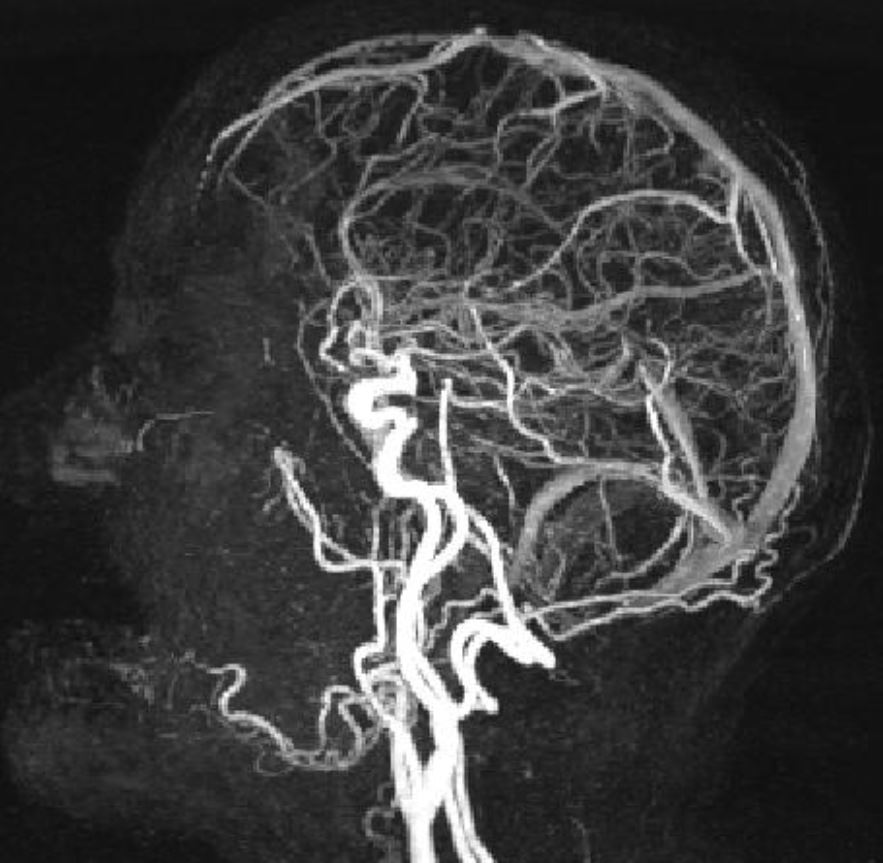
\includegraphics[width=11cm]{1_7_contrast_angiography}
\caption{Illustration d'angiographie IRM par injection de produit de contraste. Séquence SPARSE acquise sur une IRM 3T avec une antenne 20 canaux, $T_E$/$T_R$=1.37/3.28 ms, matrice = 384, détection du contraste : carbolus axial, débit = 2cc/s (12cc), agent de contraste : Dotarem, taille du voxel = 0.7 x 0.7 x 0.7 mm$^3$. L'image est une projection des intensités maximales selon le plan sagittal. }
\label{fig:1_7_contrast_angiography}	
\end{figure}
%%%
L’injection d’un produit de contraste permet, comme son nom l’indique, d’améliorer le contraste entre les tissus. Il a pour but d’augmenter le signal d’un type de structure en particulier. Le principe repose sur l’utilisation de substances paramagnétique ou super paramagnétique qui vont réduire le temps de relaxation longitudinal (T1) et transversal (effet $T_2$*) des tissus avoisinant, permettant ainsi la création d’un signal plus important en $T_1$. L’environnement interne du cerveau étant très stable, ceci est autorisé par la présence d’une barrière appelée barrière hémato encéphalique limitant le passage de certaines molécules du compartiment sanguin au liquide cérébrospinal et au liquide extracellulaire du parenchyme cérébral. La présence de cette barrière va ainsi limiter le produit de contraste au compartiment vasculaire après injection intravasculaire, ce qui permet d’apprécier l’architecture vasculaire\footnote{Notons tout de même que la diffusion du produit de contraste à l’extérieur du compartiment vasculaire reste néanmoins possible (et souvent utilisée comme critère diagnostique) dans le cadre de pathologies (gliomes) modifiant la barrière hémato-encéphalique.}.

Afin d’imager correctement le produit de contraste, les séquences adaptées imposent une synchronisation précise par rapport à l’injection du bolus pour que l’acquisition coïncide avec le passage intravasculaire du produit. Le couplage de ce type d’acquisition à des techniques d’accélération des séquences (acquisition parallèle, acquisitions partielles de l’espace K corrélées dans le temps …) permettent d’aboutir à une imagerie 4D des vaisseaux : c’est la CEMRA (« Contrast Enhanced Magnetic Resonnance Angiography »). Dans ce cas, les premiers volumes avant rehaussement servent de masque de soustraction pour extraire l’arbre vasculaire des images suivantes. Si la durée d’acquisition est suffisamment longue, les artères puis les veines seront visibles.

Ces approches souffrent actuellement de leur faible résolution, inhérente aux grandes vitesses d’acquisitions. Cette difficulté peut cependant être surmontée. Les images IRM telles que les angiogrammes contiennent en effet des informations très localisées : les pixels contenant de l’information sont relativement rares dans l’espace 3D. On a des matrices 3D creuses (« sparse »). Au vue des récents développements dans la théorie mathématique des acquisitions compressées (« compressed-sensing »), les images possédant une représentation de ce type peuvent être reconstruites à partir d’un sous-échantillonnage aléatoire de l’espace réciproque (\cite{Lustig2007}). En effet, le passage de cet échantillonnage vers l’espace image se traduit par un bruit aléatoire qui se neutralise, tandis que l’information d’intérêt, regroupée en cluster (artères etc.) ressort clairement. Ce type d’acquisition permet de l’obtention de cartographies vasculaires avec un excellent niveau de détail (Figure~\ref{fig:1_7_contrast_angiography}).


%%%
%%%
\subsection{Système artériel : imagerie par temps de vol}
%%%
\begin{figure}[!t]
\centering
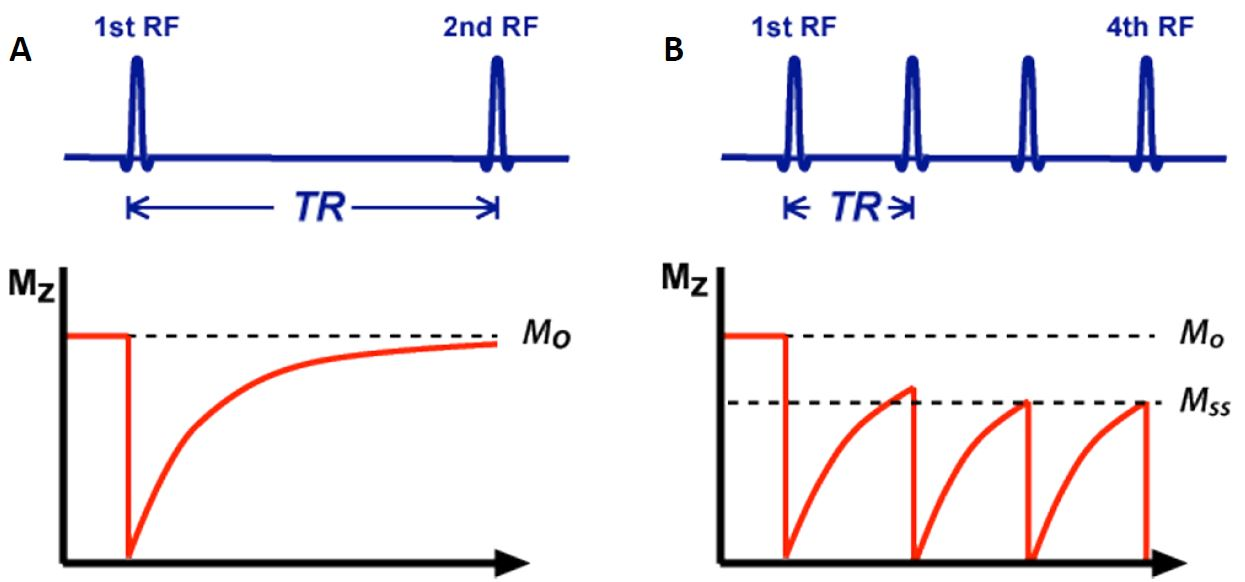
\includegraphics[width=13cm]{1_9_saturation_partielle}
\caption{Saturation partielle et développement de l'état d'équilibre d'aimantation. A) $T_R  >> T_1$ permettant une relaxation complète de l'aimantation avant la 2ieme impulsion RF. B) $T_R$ court, l'aimantation $M_z$ ne peut récupérer avant l’impulsion suivante, ce qui se traduit par l’apparition d’un nouvel état d’équilibre de l'aimantation (M$_{ss}$ , avec M$_{ss}$ < M$_{0}$) après quelques impulsions. }
\label{fig:1_9_saturation_partielle}	
\end{figure}
%%%
L’{\em imagerie par temps de vol} ("Time Of Flight" ou TOF) est une technique d’acquisition sans injection de produit de contraste permettant de mettre en évidence les flux artériels en utilisant les modifications liées au déplacement du volume sanguin, qui ne sera pas soumis à l’ensemble des impulsions radiofréquences contrairement au tissu stationnaire. Ce phénomène, appelé phénomène d’{\em entrée de coupe}, s'obtient en jouant sur la dynamique de la saturation magnétique, {\em via} les valeurs relatives du temps de répétition $T_R$ de l'impulsion radiofréquence et du temps de relaxation $T_1$. Lorsque les impulsions radiofréquences (90°) sont suffisamment éloignées ($T_R > 5  T_1$) l'aimantation longitudinale a le temps de retrouver son état initial (voir Figure~\ref{fig:1_9_saturation_partielle}) avant la prochaine impulsion. En revanche, lorsque les impulsions sont très rapprochées, cette aimantation ne peut revenir à son état initial, et une plus faible aimantation longitudinale sera disponible pour les impulsions suivantes. Après l'impulsions RF, un nouvel état d’équilibre moyen apparait (Figure~\ref{fig:1_9_saturation_partielle}) à un niveau inférieur au niveau original, c’est la saturation magnétique (voir pour une explication très claire le site ~\cite{timeflighteffects}).

Dans une imagerie par temps de vol, les tissus stationnaires sont saturés grâce à des $T_R$ très courts, ce qui conduit à une diminution de leur signal, et induit le phénomène d’entrée de coupe. En effet, comme le sang artériel circulant entrant dans la zone explorée n’a pas été saturé, son aimantation longitudinale est maximale. Le signal du sang entrant apparait alors comme plus important que celui du tissu stationnaire (Figure~\ref{fig:1_8_IRM_temps_de_vol}). La visualisation des structures artérielles peut être ensuite améliorée lors du traitement de l'image par projection des intensités maximales selon différents angles afin d’aboutir à une « pseudo » vue 3D.

Du fait du principe de l’imagerie TOF, la qualité de l’image récupérée va dépendre des caractéristiques des vaisseaux et des flux sanguins. Ainsi des flux lents (inférieurs à 10 cm/sec) (\cite{Offerman2011})  ou orientés parallèlement au plan de coupe entrainent une perte de signal de même que les flux turbulents (sténoses) (\cite{Bradley1984}). C’est la raison pour laquelle cette modalité est peu adaptée au système veineux.

%%%
\begin{figure}[!t]
\centering
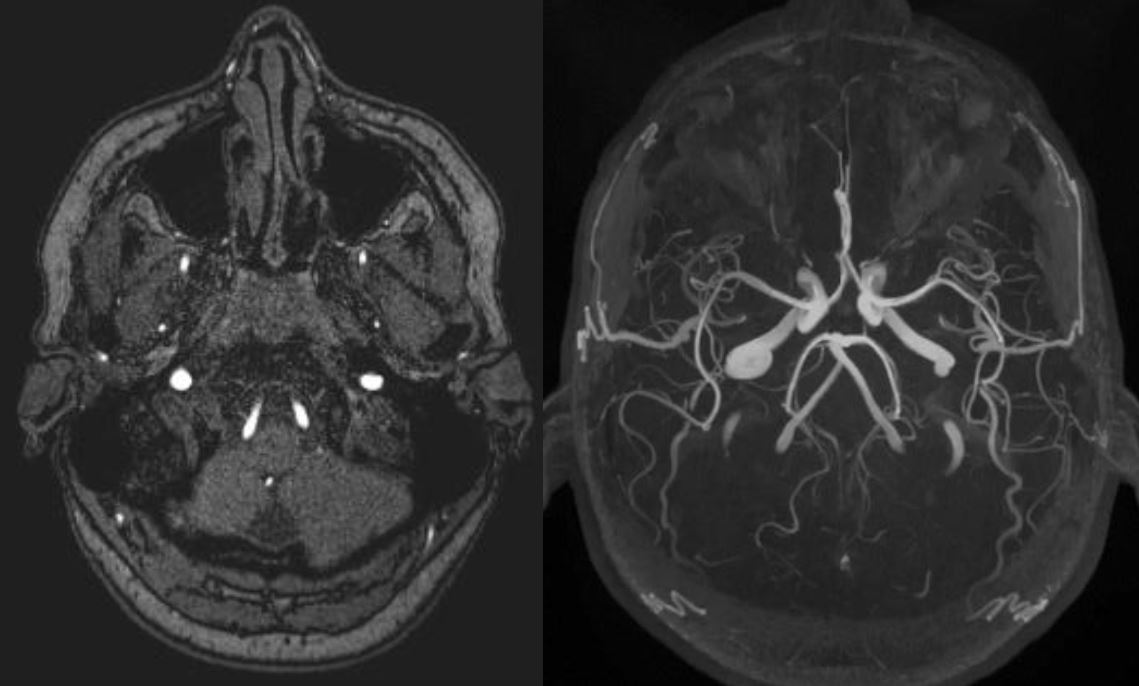
\includegraphics[width=14cm]{1_8_IRM_temps_de_vol}
\caption{Exemple d'image d'IRM par temps de vol. Le sang entrant dans le volume à imager apparait en hyper signal. A gauche l’image brute, à droite une projection des intensités maximales. La projection est obenue en identifiant le long de l'axe Z en chaque pixel(x,y) l'intensité maximale, le tout étant donc représenté dans une vue 2D. Séquence en temps de vol 3D obtenue à 3T (antenne 32 canaux) avec les paramètres : $T_E/T_R$ = 3.43/21 ms, angle de bascule = 18°, taille du voxel = 0.26 x 0.26 x 0.6 mm$^3$, 220 coupes, temps d'acquisition = 6 min.}
\label{fig:1_8_IRM_temps_de_vol}	
\end{figure}
En fonction du contexte, l’acquisition peut être 2D ou 3D. Lors d’une acquisition 2D un ensemble de coupes fines est effectué pour aboutir à un pseudo-volume 3D. Les coupes fines autorisent une meilleure sensibilité aux flux lents du fait du temps plus court passé dans la coupe. En effet les flux lents subissent l'effet de saturation de façon similaire au tissu stationnaire, l'utilisation de fines coupes permet de limiter cet effet, le sang ayant le temps de traverser ce petit volume. En contrepartie, la résolution spatiale dans l’axe de la pile de coupe est limitée. Les acquisitions 3D autorisent elles l’obtention d’une bonne résolution spatiale dans les 3 directions, ainsi qu’un meilleur rapport signal sur bruit. En revanche les flux lents risquent d’être peu voir non visibles.

Cette séquence permet donc une {\em très bonne visualisation des artères principales du cerveau} (artères cérébrales moyennes, antérieurs et postérieurs), la visualisation des artères communicantes ou des veines en revanche peut s’avérer plus compliquée du fait de leur orientation et des débits relativement faibles attendus.
%%%
%%%
\subsection{Système artériel et veineux : imagerie en contraste de phase}
L’{\em imagerie en contraste de phase} repose sur le déphasage des spins mobiles soumis à un gradient bipolaire. Pour un gradient bipolaire d’une intensité et d’une durée donnée, les spins mobiles vont se déphaser en fonction de leur vitesse.

Le gradient est orienté de telle façon à ce qu’il soit parallèle au vaisseau d’intérêt. Ainsi lors d’une première acquisition, les spins mobiles se déphasent d’autant plus que leur vitesse est grande dans le vaisseau tandis que les spins immobiles présentent un déphasage fixe. Puis, dans un second temps, les lobes du gradient d’encodage sont inversés et une seconde acquisition est réalisée. Ainsi par soustraction des deux images, le déphasage des spins stationnaires dû aux hétérogénéités de champ sera identique dans les deux acquisitions et s’annulera, tandis que les spins mobiles vont accumuler deux déphasages de sens opposés que la soustraction va cumuler (Figure~\ref{fig:1_10_principe_contraste_phase}).

%%%
\begin{figure}[!t]
\centering
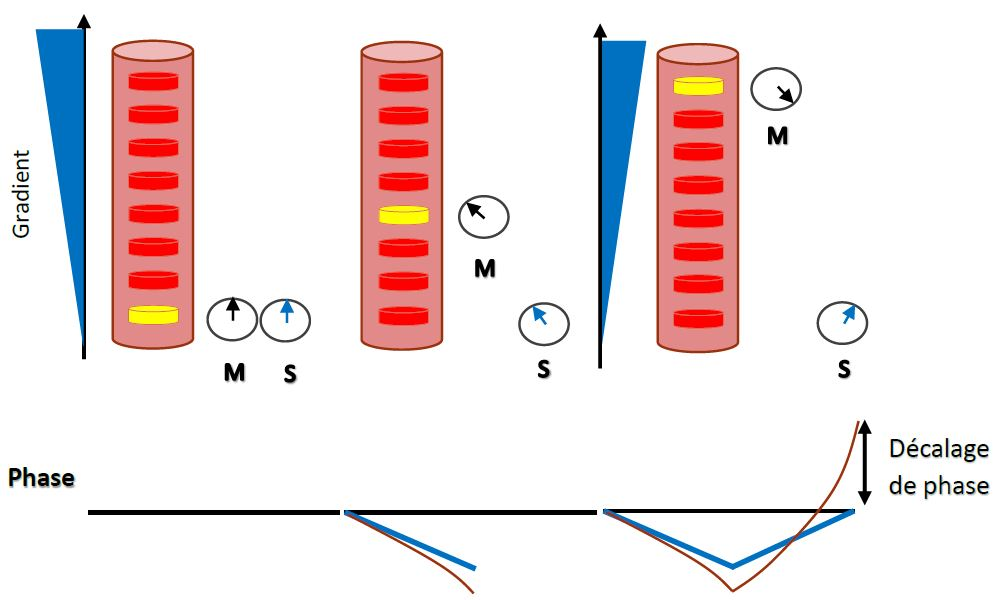
\includegraphics[width=13cm]{1_10_principe_contraste_phase}
\caption{Principe du contraste de phase. En bleu à gauche est représenté le gradient, en rouge clair le vaisseau exploré, et sous forme de disques rouge les spins sanguins. Le spin mobile (M) pris en référence est en jaune. Les spins se déplaçant dans le vaisseau le long du gradient se déphasent de façon d’autant plus importante que leur vitesse est élevée. Après l’inversion des lobes du gradient d’encodage, le déphasage du spin immobile devient nul par rapport à l’état initial, tandis que le spin mobile lui présente un décalage. }
\label{fig:1_10_principe_contraste_phase}	
\end{figure}
Pour étudier les mouvements dans toutes les directions de l’espace, on répète ceci avec des gradients d’encodage de flux dans chacune des trois directions de l’espace. Une acquisition supplémentaire sans gradient d’encodage de flux sert de référence. Les séquences employées sont de type écho de gradient.

Cette technique permet de mesurer de façon relative la vitesse et la direction des flux grâce à l’information de phase. Les flux se dirigeant vers l’examinateur sont codés en blanc, ceux s’en éloignant en noir. On peut ici mesurer des flux plus lents qu’en imagerie par temps de vol (inférieur à 10 cm/sec) pour une durée d'acquisition de 6 min 15 sec. Le contraste obtenu est adapté en particulier à la reconstruction du système veineux. Notons que que cette séquence n'est pas compensée de l'accélération, on considère que celle-ci est constante.

Les images obtenues permettent de visualiser l’ensemble des vaisseaux (Figure~\ref{fig:1_11_exemple_contraste_phase}).

%%%
%%%
\subsection{Système veineux : Imagerie de susceptibilité magnétique}
\label{sec:QSM_chap_2}
Une autre technique mettant en relief de nouveaux contrastes plus fins a été développée plus récemment: l’{\em imagerie de susceptibilité}. Définissons la susceptibilité $\chi_m$ : la plupart des matériaux placés dans un champ magnétique possèdent la capacité de s’aimanter sous l’action de ce  champ. 
\begin{equation}
\bold{M}\,=\,\chi_m\,\bold{B}_0.
\end{equation}
On distingue deux comportements différents. Certains comme l’eau, le cuivre ou le zinc, vont s’{\em opposer au champ}, entrainant une diminution de la densité des lignes de forces : on les appelle {\em diamagnétiques} (leur susceptibilité est {\em inférieure à 0}). D’autres au contraire vont se{\em placer dans le sens due champ} (air, fer, magnésium), induisant un accroissement de la densité des lignes de forces : ce sont les substances {\em paramagnétiques} (susceptibilité {\em supérieure à 0}). Notons cependant que dans le cadre de substances superparamagnétiques, que nous n'évoquerons pas ici, cette équation n'est plus valable.

A l’intérieur du cerveau coexistent des substances possédant différentes propriétés vis-à-vis de l'aimantation : certaines structures vont ainsi être plutôt diamagnétique (myéline) ou paramagnétique (veines, pallidum ; \cite{Wang_Liu_2014}). La possibilité de mesurer quantitativement cette susceptibilité a été évoquée dès les premières années de l’imagerie IRM (\cite{Young1987}). Les variations locales de la susceptibilité engendrent des variations locales concomitantes du champ magnétique effectif subit par le matériau, qui vont engendrer des distorsions locales des lignes de champ et ainsi des décalages en fréquence localisés. Les variations de susceptibilités sont donc à première vue des source d’{\em artéfacts}.  
Depuis une quinzaine d'années a été développée une première modalité d’imagerie sensible aux variations de susceptibilité : l’{\em imagerie pondérée en susceptibilité} (Susceptibility Weighted Imaging ou SWI; \cite{Reichenbach2001}). Cette méthode tente d’utiliser l’information portée par l’imagerie de phase afin de fournir un contraste nouveau sensible en particulier aux veines et autres structures disposant d’une forte susceptibilité (cavernomes, calcifications etc.). En effet la saturation en oxygène dans le système veineux étant faible, le sang veineux est riche en dé-oxyhémoglobine, molécule disposant d’une forte susceptibilité. De ce fait cette imagerie donne accès au système veineux et ce potentiellement avec une résolution légèrement plus fine que le contraste de phase (0.6 mm isotropique contre 0.47 x 0.47 x 1 mm$^3$) pour un temps d'acquisition similaire (6 à 7 min). En susceptibilité  l'information récupérée ne dépend pas de l'orientation de gradients, aucun gradients d'encodage de flux n'est utilisé. Cela permet d'avoir accès aux veines peut importe leur orientation (\cite{Fan2014}). L'ensemble conduit à avoir accès à des veines plus petites. En revanche l’image ne contient pas que des vaisseaux, toutes les structures présentant une susceptibilité importante et du fait de la magnitude, les autres tissus. Il reste cependant possible d’extraire une partie des veines de l’image via des algorithmes dédiés (\cite{Manniesing2006}) avec plus ou moins de succès.

%%%
\begin{figure}[!t]
\centering
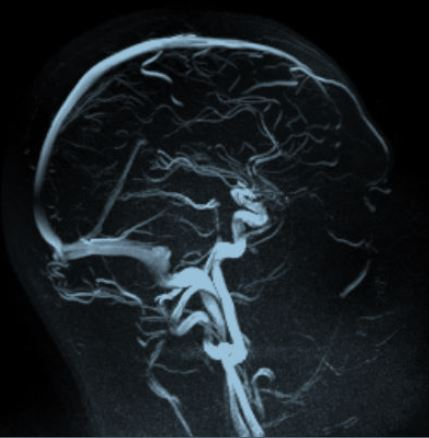
\includegraphics[width=9cm]{1_11_exemple_contraste_phase}
\caption{Exemple d'image de contraste de phase (projection). Paramètres: champ de vue 24 x 24 cm, temps d’écho = 7.91 ms, temps de répétition = 35.7 ms, angle de bascule = 15°, taille de voxel = 0.47 x 0.47 x 1 mm$^3$, 144 niveaux de coupes, temps d'acquisition = 6 min.}
\label{fig:1_11_exemple_contraste_phase}	
\end{figure}

Rappelons que lors d’une acquisition standard en IRM, le signal récupéré est codé sous forme complexe, et contient donc deux informations : partie imaginaire et partie réelle. Le plus usuellement ces deux informations sont combinées pour générer une imagerie de magnitude correspondant à la racine de la somme du carré des parties réelles et imaginaires :
\begin{equation}
M\,=\sqrt[2]{\,Re^2\,+\,Im^2}.
\end{equation}
Cette image de magnitude est la plus utilisée en IRM pour le diagnostic. Elle permet de maximiser le rapport signal sur bruit et fournit le meilleur contraste anatomique. L’image de phase, elle, est obtenue en calculant la tangente inverse du rapport partie imaginaire sur partie réelle :
\begin{equation}
\Phi\,=\,atan\biggl(\frac{Re}{Im}\biggr).
\end{equation}
Cette imagerie de phase reflète directement les déphasages dû à la variabilité de la susceptibilité magnétique et donc du champ. Ces mêmes effets se traduisent par une perte de signal dans l’imagerie de magnitude. L'image de SWI combine ces deux informations selon une pondération arbitraire conduisnat au peilleur rendu visuel. 

La séquence correspondante elle-même est une séquence en {\em écho de gradient} standard. Le paramètre important est ici le temps d’écho. En effet, un temps d’écho court (inférieur à 20 ms) limitera la présence d’artéfacts mais réduira la visibilité des faibles susceptibilités, tandis que un temps d’écho long (supérieur à 20 ms) favorisera la détection de petites lésions hémorragiques et par la même occasion augmentera les artéfacts de l’image liés aux très fortes susceptibilités (\cite{Kressler2010}). Bien qu’un temps d’écho unique suffise à générer une cartographie pondérée en susceptibilité, il est bon de noter que de nouvelles approches à multi temps d’échos se développent afin de limiter la présence d’artéfacts dans l’image (\cite{Oh2013}). Les séquences peuvent être trouvées chez la plupart des constructeurs sous différents acronymes : SWI, SWAN, PADRE.

Néanmoins, en imagerie pondéré en susceptibilité magnétique l’apport de l’image de phase n’est comme on l'a noté que qualitatif, cette dernière servant seulement de facteur multiplicatif à l’imagerie de magnitude (voir détails chapitre~\ref{chap:qsm}).

Plus récemment, une nouvelle technique intitulé {\em cartographie quantitative de susceptibilité} (Quantitative Susceptibility Mapping : QSM) a été développée avec l’ambition de remonter aux valeurs physiques exactes de la susceptibilité locale. En effet, la capacité à estimer quantitativement et non plus qualitativement a un nombre important d’applications potentielles. Comme on l'a dit, de nombreux tissus possèdent des susceptibilités différentes de leur environnement. Le calcium par exemple, possède une susceptibilité négative (diamagnétique) par rapport à l’eau. La mesure de susceptibilité pourrait ainsi permettre de mesurer la densité minérale de l’os (\cite{Chung1996}). Nous pouvons aussi mentionner, parmi les applications possibles : la différenciation des calcifications et des hémorragies chroniques (\cite{Kozic2009}), la mesure de la perte de myéline (\cite{Liu2011}), la quantification de la CMRO2 (\cite{Zhang2014}), ou encore la mesure de la saturation en oxygène dans les veines (\cite{Fan2014}).

Nous développerons au chapitre~\ref{chap:qsm} les difficultés intrinsèques à la reconstruction de cette susceptibilité. Pour résumer, la difficulté est double, reconstruire le champ à l’intérieur de l’espace intracrânien, puis à partir de ce champ obtenir la carte de susceptibilité. Ce problème est analytiquement mal posé et doit être abordé à l’aide de techniques numériques sophistiquées (\cite{Haacke2005},\cite{Shmueli2009}). Ce caractère mal posé conduit à la présence persistante d’artéfacts dans la carte de susceptibilité reconstruite. En l’état de l’art ces artéfacts ont été maîtrisés de façon suffisante pour faire émerger la QSM dans le domaine de la recherche clinique (\cite{Wang_Liu_2014}, \cite{Bilgic2013}, \cite{Deistung2013}).

En résumé, nous utiliserons principalement cette technique pour raffiner la reconstruction du système veineux fournit par le contraste de phase (Figure \ref{fig:1_12_image_QSM}). En effet, la résolution plus fine de la carte de susceptibilité magnétique et son aspect quantitatif vont permettre de visualiser de plus petites veines et de les extraire facilement par simple seuillage sur la base de la valeur en $ppm$.
%%%
\begin{figure}[!t]
\centering
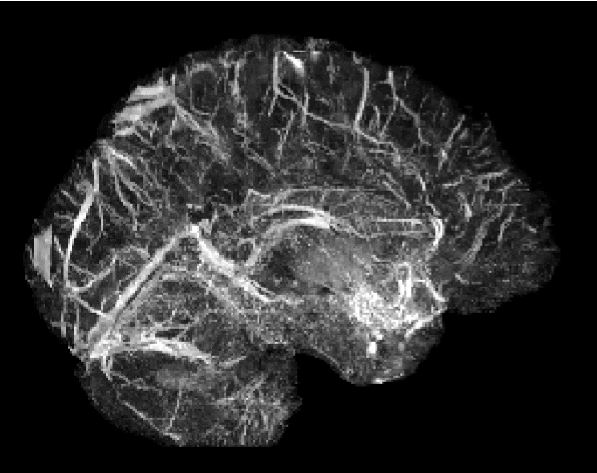
\includegraphics[width=12cm]{1_12_image_QSM}
\caption{Image de QSM obtenue après projection des intensités maximales. On met en évidence ici les veines pouvant être obtenues par simple seuillage. Notons que les sinus veineux en périphéries sont peu visibles du fait de l’érosion réalisée sur cette image (voir~\ref{sec:calcsusc}). Résolution 0.6 x 0.6 x 0.6 mm$^3$.}
\label{fig:1_12_image_QSM}	
\end{figure}

%%%
%%%
\subsection{Mise en place d'un protocole d'acquisition}
Compte tenu du cahier des charges défini dans l’introduction, la construction d’un modèle quantitatif détaillé adapté à la morphologie de chaque patient doit s’appuyer sur deux groupes d’informations. Les informations {\em morphologiques} correspondent à l’architecture du réseau artériel et du système veineux du patient, et les volumes de matière grise, blanche et du liquide cérébro-spinal du patient.

Nous avons donc défini un protocole d’acquisition IRM dédié à l’implémentation de ce modèle qui incorpore toutes les séquences nécessaires à la collecte de ces informations au vue de l’état de l’art et des contraintes techniques de nos appareils. Nous faisons le choix, de n’utiliser que des séquences non-injectées afin de ne limiter le protocole à aucune catégorie de patients. Néanmoins, dans le cadre de la validation du modèle,  nous n’excluons évidemment pas d’utiliser dans certains cas particuliers des protocoles avec injection. Les données d’imagerie IRM ont été recueillies sur une IRM 3 tesla (Skyra, Siemens, Allemagne) en utilisant une antenne tête 32 éléments. Ces séquences sont bien définies dans la littérature et communes, nous ne discuterons donc pas le détail de chacun des paramètres. La SWI fera cependant exception, le détail et les justifications étant données dans un chapitre dédié (chapitre~\ref{chap:qsm}).

Concernant les informations morphologiques, le protocole inclut les imageries anatomiques suivantes :
\begin{itemize}
\item un 3DT1 pour récupérer les volumes de matière grise, de matière blanche et de LCS, acquis avec les paramètres suivants : champ de vue = 25 x 25 cm, temps d’écho = 2.5 ms, temps de répétition = 1690 ms, angle de bascule = 9°, taille de voxel = 0.98 x 0.98 x 1 mm$^3$, 176 niveaux de coupes, temps d'acquisition = 4 min ;
\item un temps de vol artériel pour accéder à l’architecture artérielle, avec les paramètres : champ de vue 18.1 x 20 cm, temps d’écho = 3.43 ms, temps de répétition = 21 ms, angle de bascule = 18°, taille de voxel = 0.26 x 0.26 x 0.6 mm$^3$, 220 niveaux de coupes,  temps d'acquisition = 6 min ; avec une couverture suffisante pour imager jusqu’à la partie supérieure de l’artère cérébrale antérieure
\item un contraste de phase qualitatif pour récupérer le compartiment veineux avec les paramètres : champ de vue 24 x 24 cm, temps d’écho = 7.91 ms, temps de répétition = 35.7 ms, angle de bascule = 15°, taille de voxel = 0.47 x 0.47 x 1 mm$^3$, 144 niveaux de coupes,  temps d'acquisition = 6 min ;
\item une imagerie quantitative de susceptibilité magnétique afin de préciser l’arborescence veineuse avec les paramètres : champ de vue 20 x 22 cm, temps d’échos = 10/20 ms, temps de répétition = 27 ms, angle de bascule = 15°, taille de voxel = 0.69 x 0.69 x 0.6 mm$^3$, 224 niveaux de coupes,  temps d'acquisition = 6 min 30 sec ; avec sauvegarde des raw data.
\end{itemize}
Comme nous l’avons vu l’arbre vasculaire est un système complexe. Il convient donc de définir clairement à quel niveau nous souhaitons nous placer afin de définir les entrées et sorties utilisées. Le sang entre dans le cerveau principalement par quatre voies : les deux carotides internes et les artères vertébrales. Ces artères vertébrales se rejoignent pour former l’artère basilaire. Ainsi pour limiter la complexité du système nous avons choisi de positionner notre boite d’acquisition de telle sorte à ce que le premier niveau de coupe intègre les {\em deux carotides} et l’{\em artère basilaire}, pour un total de trois entrées. De plus l’artère basilaire sera plus visible du fait de son diamètre et donc plus facilement segmentable en comparaison des artères vertébrales. En terme de sorties, nous récupèrerons à ce niveau les deux {\em veines jugulaires}.

%%%
\begin{figure}[!t]
\centering
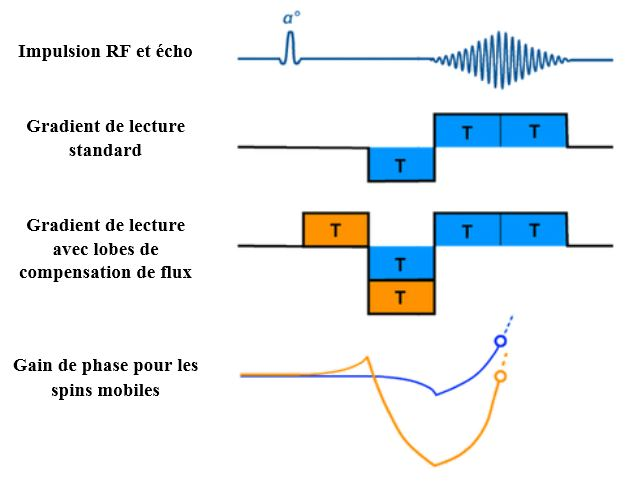
\includegraphics[width=12cm]{1_13_compensation_flux}
\caption{Exemple de la compensation de flux en IRM sur une séquence de type écho de gradient. L'impulsion radiofréquence (RF) est indiquée en première ligne, les gradients standard en seconde ligne, la troisième ligne présente en orange les lobes additionnels pour la compensation de flux. L'évolution de la phase pour les spins mobiles apparait en dernière ligne, sans compensation de flux (bleu) et avec (orange). Sans compensation, la phase des spins mobiles est positive. Avec compensation la phase au centre de l'écho est nulle (\cite{flowcompensation}). }
\label{fig:1_13_compensation_flux}	
\end{figure}

%%%
%%%
Enfin il est important d'évoquer un dernier point relatif à l'imagerie des vaisseaux : la compensation de flux. Dans les séquences d'imagerie classiques (excepté le contraste de phase), la phase des spins est censée correspondre à une information spatiale uniquement (codage de phase). Un gradient bipolaire dont les deux lobes positifs et négatifs sont de même importance n'a pas d'effet sur la phase des spins stationnaires. En revanche, si un spin est en mouvement dans l'axe du gradient, il ne va pas subir le même effet de gradient en fonction de sa position. Par conséquent, les spins mobiles seront mal positionnés et on observera un artéfact de déplacement des structures vasculaires et des fluides en mouvement. Dans notre contexte ce genre d'artéfacts nous empêcherais d'identifier avec précision les vaisseaux. Dès la fin des années 1980, Pattany et al. (\cite{Pattany1987}) ont proposé un ajustement des gradients afin de corriger ces artéfacts ({\em Motion Artifact Suppression Technique}), connu maintenant sous le nom de {\em compensation de flux}. Dans cette approche, des lobes de gradient additionnels sont rajoutés préalablement à la lecture du signal afin de compenser les déphasages induits par les mouvements au temps d'écho. La Figure~\ref{fig:1_13_compensation_flux} illustre l'effet des lobes additionnels sur les spins mobiles. Pour les spins stationnaires, les lobes additionnels de gradient (orange) n'ont aucun effet, chacun ajoutant ou réduisant une quantité de phase constante. Puisqu'il y a deux lobes positifs et deux lobes négatifs avant le centre de l'écho, leur effet net est nul. Pour les spins mobiles, l'effet est différent. La courbe bleue indique l'évolution de la phase dans la séquence standard. Les spins mobiles accumulent une phase non nulle au centre de l'écho (cercle bleu), ce qui se traduit par une perte de signal sur l'image. L'effet des nouveaux lobes sur les spins mobiles est illustrée par la courbe orange. Le premier lobe créé un gain de phase, mais le second, lorsqu'il s'ajoute au premier lobe bleu créé une perte de phase fortement négative. Cependant la phase de ces spins devient nulle au centre de l'écho (cercle orange).

La compensation de flux peut être réalisée dans la direction de la sélection de coupe aussi bien que dans la direction de lecture. Les limitations principales de cette technique sont que : (1) elle ne corrige que du mouvement à {\em vitesse constante}; (2) le $T_E$ minimum est allongé du fait du temps requis pour ajuster les nouveaux gradients; (3) la pression sur les gradients est accrue limitant potentiellement le champ de vue ou l'épaisseur de coupe pour un $T_R$ donné; et (4) des artéfacts causés par les courants de Foucault peuvent être induit par la commutation rapide des gradients.

Afin d'améliorer la qualité de nos images morphologiques et limiter les artéfacts dans l'image, les séquences utilisées à l'exception du contraste de phase disposeront donc de compensation de flux dans deux directions voir trois si possible.

Ce protocole sera complété à la fin de la seconde partie par les modes d’imagerie donnant accès à la {\em dynamique}.





			
		
\bibliography{jeremythesebib}{}
\bibliographystyle{francaissc}